\section{Comparison of traffic engineering methods using ns-2 simulations}
%\renewcommand{\topfraction}{.7}
%\renewcommand{\bottomfraction}{.7}
%\renewcommand{\textfraction}{.3}

In this section we compare the performance of traffic engineering schemes based on application performance in the network. Our results show that difference in MLU has a minimial effect on throughput in the network. The mean download rates of different traffic engineering methods are near identical in all our datasets.

\subsection{Experiment description}
We performed the experiments in this section for 2 days of data from Abilene, Geant and US-ISP datasets.
From each day of data in Abilene , Geant and US-ISP we randomly selected 50 out of 288 , 25 out of 96 and 24 of out 24 matrices respectively. We simulated each of these traffic matrices using ns-2 and we present the aggregate results for all the traffic matrices in a day. We present the results  for 7th April 2004 for Abilene, and 23rd January 2005 for Geant. We do not have the date information for US-ISP.  The results were similar from the trafffic matrices from other day. 

We present two statistics for each Traffic Engineering scheme:
\begin{enumerate}
\item Download rate: The download rates of a file in kilobytes per second
\item Download ratio: The ratio of the download rate of a file to its rate in the Optimal MLU traffic engineering scheme
\end{enumerate}
We sort the download rate and ratios of all files during the simulation in increasing order and present them.

\subsection{Performance of TE methods for intra-domain traffic matrices on ISP Topologies}

\begin{figure*}[htb]
  \begin{center}
    \subfigure[Download rate US-ISP]{\label{fig:edge-a}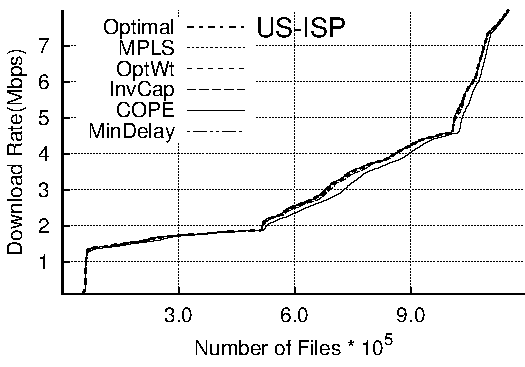
\includegraphics[scale=0.6]{newImages/ATT_download_rates_aggregate_plot.pdf}} 
    \subfigure[Download rate Geant ISP]{\label{fig:edge-a}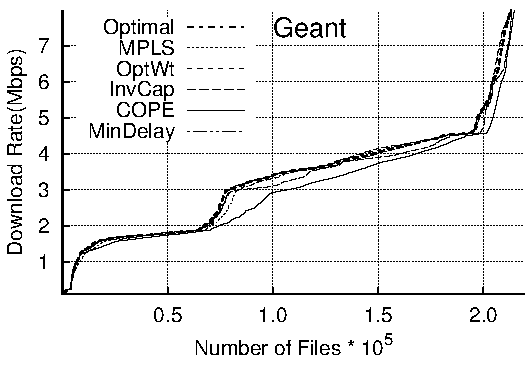
\includegraphics[scale=0.6]{newImages/Geant_download_rates_aggregate_plot.pdf}} 
    \subfigure[Download rate Abilene ISP]{\label{fig:edge-a}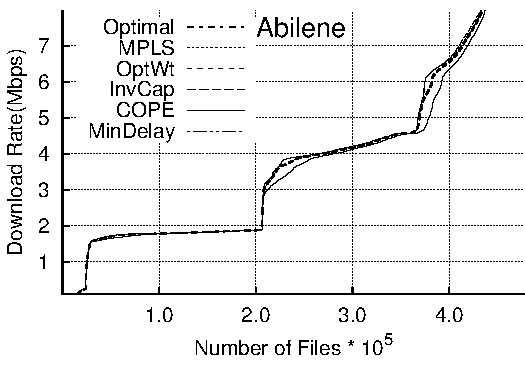
\includegraphics[scale=0.6]{newImages/Abilene_download_rates_aggregate_plot.pdf}}  
    \subfigure[Download ratio US-ISP]{\label{fig:edge-b}\includegraphics[scale=0.6]{newImages/ATT_opt_download_ratios_aggregate_plot.pdf}} 
    \subfigure[Download ratio Geant ISP]{\label{fig:edge-b}\includegraphics[scale=0.6]{newImages/Geant_opt_download_ratios_aggregate_plot.pdf}} 
    \subfigure[Download ratio Abilene ISP]{\label{fig:edge-b}\includegraphics[scale=0.6]{newImages/Abilene_opt_download_ratios_aggregate_plot.pdf}} 
  \caption{Aggregate download rate and download ratios on US-ISP, Geant and Abilene traffic matrices for 1 day traffic matrices}
  \end{center}
  \label{fig:allisps_aggregate_internetBW}
\end{figure*}


%
%\begin{figure*}[htb]
%  \begin{center}
%    \subfigure[Download rate US-ISP]{\label{fig:edge-a}\includegraphics[scale=0.4]{newImages/US_ISP/internetBW/download_rates_aggregate_plot.pdf}} 
%    \subfigure[Download rate Geant ISP]{\label{fig:edge-a}\includegraphics[scale=0.4]{newImages/Geant/internetBW/download_rates_aggregate_plot.pdf}} 
%    \subfigure[Download rate Abilene ISP]{\label{fig:edge-a}\includegraphics[scale=0.4]{newImages/Abilene/internetBW/download_rates_aggregate_plot.pdf}}  
%    \subfigure[Download ratio US-ISP]{\label{fig:edge-b}\includegraphics[scale=0.4]{newImages/US_ISP/internetBW/opt_download_ratios_aggregate_plot.pdf}} 
%    \subfigure[Download ratio Geant ISP]{\label{fig:edge-b}\includegraphics[scale=0.4]{newImages/Geant/internetBW/opt_download_ratios_aggregate_plot.pdf}} 
%    \subfigure[Download ratio Abilene ISP]{\label{fig:edge-b}\includegraphics[scale=0.4]{newImages/Abilene/internetBW/opt_download_ratios_aggregate_plot.pdf}} 
%  \caption{Aggregate download rate and download ratios on US-ISP, Geant and Abilene traffic matrices for 1 day traffic matrices}
%  \end{center}
%  \label{fig:allisps_aggregate_internetBW}
%\end{figure*}

For the traffic load in  ISP networks and the users access link distribution, the performance of traffic engineering schemes is surprisingly similar. In  Fig 2 we plot the aggregate download times and download ratios for all three datasets. In US-ISP and Abilene datasets, the median difference in download rates for all TE schemes excluding COPE is near identical. COPE has less throughput than other routings in all 3 ISPs and has approx 10 \% lower median throughput in Geant.   This is because COPE has a higher delay as shown by statistics later in this section.  We plot the mean throughputs in Fig ~\ref{fig:allisps_aggregate_mean_internetBW} for different routings. As suggested by the throughput curve, the mean throughputs except COPE differ by less than 5\%.

% COPE has 10\% lower mean throughput than other schemes in Geant.  This can also be seen from delay statistics we present later in this section.

The download ratio curves highlights the difference among schemes more clearly.  Both MplsAvg and MinDelay have nearly identical performance to Optimal for all three topologies. The small fraction of files for which they have a lesser throughput than Optimal  is offset by a nearly identical fraction of files for which these schemes have a higher throughput than Optimal.  In comparison, OspfOptWt comes next in line followed by InvCap. OspfOptWt has 10th percentile throughput approx 10\% less than Optimal and the difference decreases thereafter. The difference in download ratios is maximum for COPE. For the 10th percentile, it download ratio is more than 20\% less than Optimal for all topologies.

%Excluding COPE, different TE schemes have identical throughput for 80\% of files for both US-ISP and Abilene topologies. In Geant topology, the result is same after excluding OSPFInvCap and MPLSAvgMLU. Both MPLS Avg and Minimize Delay have nearly identical performance to MLU Optimal scheme. The small fraction of files for which they have a lesser throughput than MLU Optimal scheme is offset by a nearly identical fraction of files for which these schemes have a higher throughput than MLU Optimal.  OSPFOptWt has slightly lower performance, at 10th percentile its throughput is 90\% of the MLU optimal TE scheme and decreases thereafter. The difference in download ratios is maximum for COPE. For the 10th percentile, it download ratio is 20\%, 35\% and 20\%  less than MLUOptimal for different TE schemes.
\begin{figure}[tbh]
  \begin{center}
\includegraphics[scale=0.7]{newImages/mean_throughput_internetBW.jpg}
  \end{center}
  \caption{Mean throughputs of file transfers for 1 day traffic matrices }
  \label{fig:allisps_aggregate_mean_internetBW}
\end{figure}

%
%\begin{figure}
%\begin{center}
%  \begin{tabular}{| l | c | c | c | }
%    \hline
%Routing & Abilene & Geant & US-ISP \\ \hline \hline
%Optimal	&	400.3	&	426.3	&	486.9	\\ \hline
%OspfInvCap	&	397.1	&	410.4	&	490.8	\\ \hline
%MplsAvg	&	400.3	&	418.4	&	486.5	\\ \hline
%COPE	&	384.1	&	384.6	&	473.3	\\ \hline
%OspfOptWt	&	399.1	&	424.1	&	492.6	\\ \hline
%MinDelay	&	401.2	&	428.4	&	492.7	\\ \hline
%  \end{tabular}
%\end{center}
%\caption{Mean throughputs of file transfers for 1 day traffic matrices }
%  \label{fig:allisps_aggregate_mean_internetBW}
%\end{figure}

In every statistic, MplsAvg and OspfOptWt perform near identical to Optimal. Notably, both MplsAvg and OspfOptWt are offline TE schmes which compute routing once every 3 hours. This shows that offline TE schemes can achieve the same perfomance as online TE schemes in ISP networks today. Interestingly, OSPFInvCap performs fairly well. Our results show that its simple heuristic of sending more traffic along paths with higher capacity is a fairly good heuristic in practice. COPE's formulation tries to optimize MLU in the common case which it hurts rather than helps throughput.

\subsection{Comparison of MLU}

 We plot the MLU for the traffic matrices for all 3 ISPs  in our experiments ~\ref{fig:All_ISPs_MLU}. These values of MLU are empirical values obtained from ns-2 simulation and they match closely to the values obtained using numerical calculation. 

 For US-ISP, COPE's and MplsAvg have link utilization very close to Optimal . OspfOptWt has upto 50\% higher MLU than value and OspfInvCap has nearly twice as high MLU than the Optimal value. For the Geant topology, the absolute difference in MLU values of different TE scheme is within 0.1, except OspfOptWt which has twice as high MLU than other schemes. Abilene traffic matrices MLU of less than 0.1 for majority of traffic matrices. Few traffic matrices have higher maximum link utilization and for these matrices all TE schemes have nearly twice the MLU values than Optimal.

\begin{figure*}[htb]
  \begin{center} \subfigure[MLU US-ISP]{\label{fig:edge-a}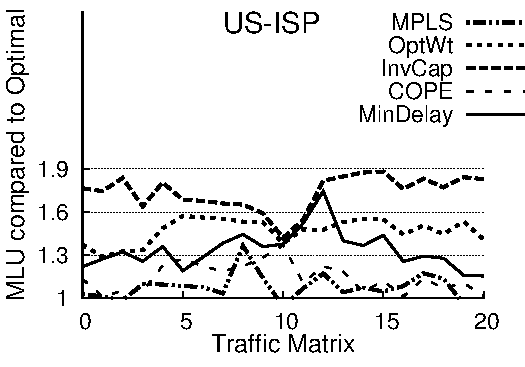
\includegraphics[scale=0.65]{newImages/ATT_MLUAverageUtilTable_plot.pdf}}
\subfigure[MLU Geant]{\label{fig:edge-a}\includegraphics[scale=0.65]{newImages/geant_plot.pdf}}
\subfigure[MLU Abilene]{\label{fig:edge-a}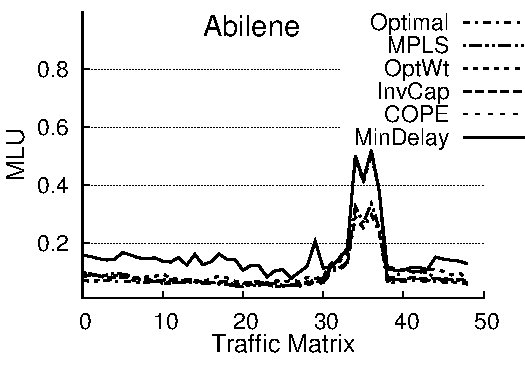
\includegraphics[scale=0.65]{newImages/Abilene_MLUAverageUtilTable_plot.pdf}}
  \end{center}
  \caption{MLU from ns-2 simulations for all traffic matrices - US-ISP, Geant and Abilene }
  \label{fig:All_ISPs_MLU}
\end{figure*}

The contrast between MLU and throughputs graph is stark. OspfInvCap has twice the MLU over Optimal scheme for US-ISP but its mean throuhput is near the same. Similarly, OspfOptWt has 50\% higher MLU over the  Optimal in Geant and US-ISP data but its throughput is near identical. COPE has a MLU within 0.1 of  Optimal but its throughput is the lowest among all TE schemes. Another related observation is that Optimal does not have an advantage over other TE schemes for throughput. %This reiterates our intial observation that MLU Optimal is not throughput Optimal.

The results can be explained by the relation between TCP throughput and link utilization. Higher link utilizations cause increased loss rates and higher queuing delay for packets. We find that in our experiments both these values remain near-zero until link utilization values of 0.6 in our experiments. Since the MLU on most of the traffic matrices are below this threshold value, MLU isnt a factor in the throughput of file downloads. Even if the utilization on one link is high enough to increase loss rates on that link the rest of the network may not be facing any congestion. File downloads rates are affected only for flows on this link, which could a small fraction of total number of file downloads.

It must be noted that our experiments are at scale 1:10 to 1:50. At, higher scale the loss rate and queuing delay would be lower at the same link utilization level. As scale increases, the router buffer sizes increase and the per packet processing time decrease proportionally. If we take the analogy from a queuing model such as $M/M/1/K$ queue, at higher loads the mean packet arrival rate ($\lambda$), the mean packet processing rate($\mu$) and the capacity of the queue ($K$) increase proportionately. The formula for loss rates of this queuing model show that both these metrics decrase as $\lambda$, $\mu$  and $K$ increase proportioately \cite{queue}. If anything , the scale of our experiments reinforces our results that MLU has minimal application performance in realistic ISP topologies. Later in this section we show some experiments at higher scale to validate our hyopthesis.

\subsection{Comparison of propagation delay}

In Fig ~\ref{fig:prop_delay_all}, we present the average propagation delay for TE methods. The propagation delays presented are the average propagation delay for all file transfers.  The notable outlier in the table is COPE which has the highest delay in all three topologies. It delay is maximum in Geant where it has 25\% higher delay than the next highest delay TE method. This explains the the reason for COPE having lower throughput than other TE schemes. All other TE methods have delay within 1ms of each other for Abilene and US-ISP. Their near identical througputs reflect this trend.

We calculate this statistic from the traffic matrix and routing computed by a TE method. First, we calculate the delay of tranfers between a source destination pair by multiplying the propagation delay by the total traffic on each path. The sum of this delay for all source destination pairs gives the total delay for a traffic matrix. The total propagation delay is the sum of delays of all trafic matrices divided by the sum of all traffic matrices.


\begin{figure}
\begin{center}
  \begin{tabular}{| l | c | c | c | }
    \hline
Routing & Abilene & Geant & US-ISP \\ \hline \hline
Optimal &  4.54 &	9.46 & 9.37\\ \hline
InvCap & 4.13 &10.62 & 9.90 \\ \hline
MplsAvg & 4.58 & 9.40 & 9.37\\ \hline
COPE &4.97 & 14.38 & 11.03\\ \hline
OspfOptWt & 3.98 & 9.57 & 9.64\\ \hline
MinDelay & 3.97 & 7.34 & 9.21\\ \hline
  \end{tabular}
\caption{Propagation delay (in ms) for TE methods on different topologies}
\end{center}
\label{fig:prop_delay_all}
\end{figure}

\subsection{Effect of access link bottlenecks}

We measure the effect of access link capcity of users on our results by experimenting at higher capacity access link bottlenecks. A reasonable choice for higher access link bottleneck is doubling current the access link capacities. In Table ~\ref{fig:all_isps_internetBWx2} shows the mean throughputs for all 3 ISPs. The mean throghputs increase by 1.3-1.7 times but the relative difference between different routings remain the same. This shows that throughputs of different traffic engineering schmes are near identical because of current traffic load in the network and would remain identical even if the current internet bandwidths were much higher.

\begin{figure}[tbh]
  \begin{center}
\includegraphics[scale=0.7]{newImages/mean_throughput_twice_internetBW.jpg}
  \end{center}
  \caption{Mean throughputs of file transfers at twice internet access link bandwidths}
  \label{fig:all_isps_internetBWx2}
\end{figure}

%\begin{figure}
%\begin{center}
%  \begin{tabular}{| l | c | c | c | }
%\hline
%Routing & Abilene & Geant & US-ISP \\ \hline \hline			
%Optimal	&	589.5	&	720.6	&	671.1	\\ \hline
%OspfInvCap	&	580.6	&	721.9	&	640.1	\\ \hline
%MplsAvg	&	589.4	&	720.0	&	654.1	\\ \hline
%COPE	&	560.4	&	695.4	&	587.8	\\ \hline
%OspfOptWt	&	586.2	&	723.1	&	662.2	\\ \hline
%MinDelay	&	589.8	&	723.9	&	663.9	\\ \hline
%  \end{tabular}
%\caption{Mean throughputs at twice the internet access link bottlenecks}
%\end{center}
%\label{fig:all_isps_internetBWx2}
%\end{figure}

\begin{figure*}[htb]
  \begin{center}
    \subfigure[Download rate US-ISP]{\label{fig:edge-a}\includegraphics[scale=0.4]{newImages/US_ISP/internetBW_scale2/download_rates_aggregate_plot.pdf}} 
    \subfigure[Download rate Geant ISP]{\label{fig:edge-a}\includegraphics[scale=0.4]{newImages/Geant/internetBW_scale2/download_rates_aggregate_plot.pdf}} 
    \subfigure[Download rate Abilene ISP]{\label{fig:edge-a}\includegraphics[scale=0.4]{newImages/Abilene/internetBW_scale2/download_rates_aggregate_plot.pdf}}  
    \subfigure[Download ratio US-ISP]{\label{fig:edge-b}\includegraphics[scale=0.4]{newImages/US_ISP/internetBW_scale2/opt_download_ratios_aggregate_plot.pdf}} 
    \subfigure[Download ratio Geant ISP]{\label{fig:edge-b}\includegraphics[scale=0.4]{newImages/Geant/internetBW_scale2/opt_download_ratios_aggregate_plot.pdf}} 
    \subfigure[Download ratio Abilene ISP]{\label{fig:edge-b}\includegraphics[scale=0.4]{newImages/Abilene/internetBW_scale2/opt_download_ratios_aggregate_plot.pdf}} 
  \caption{US Tier 1 ISP, Aggregate performance on 1 day traffic matrices,twice today's internet access link bottleneck distribution }
  \end{center}
  \label{fig:allisps_aggregate_internetBWX2}
\end{figure*}

As an interesting aside, we present the results for no access link bottlenecks in Fig  ~\ref{fig:allisps_aggregate_nolimit} .

\begin{figure*}[htb]
  \begin{center}
\subfigure[US-ISP]{\label{fig:edge-c}\includegraphics[scale=0.75]{newImages/ATT_nolimit_Download_ratio_aggregate_plot.pdf}}
\subfigure[Geant]{\label{fig:edge-c}\includegraphics[scale=0.75]{newImages/Geant_nolimit_Download_ratio_aggregate_plot.pdf}}
\subfigure[Abilene]{\label{fig:edge-c}\includegraphics[scale=0.75]{newImages/Abilene_nolimit_Download_ratio_aggregate_plot.pdf}}
  \end{center}
  \caption{All ISPs : Download ratios for 1 day traffic matrices, without access link bottlenecks}
  \label{fig:allisps_aggregate_nolimit}
\end{figure*}

%\subsection{Experiments at higher scale}
%As said previously in this section, our simulations at lower scale provide a more challenging environment for comparison. To experimentally validate our findings at a higher scale, we selected 5 traffic matrices from each ISP and repeated our simulation at a higher scale. We simulated Abilene and Geant topology at original scale and the US-ISP topology at scale 1:10. We present the aggregate download ratios for 5 traffic matrices for at scale 1:50 and scale 1:10. The download ratios curve highlight the difference between traffic engineering schmes more clearly. The shape of the curves look almost the same in both graphs. This shows that our results remain consistent even at higher scale.
%
%Thus our results for 3 ISPs based on ns-2 simulations show that under traffic conditions in the internet the throughput performance of all traffic engineering schemes differ are near identical. Our results are consistent even at higher acess link botttlenecks in the internet and on experiment at higher scale. These findings show that difference in MLU for TE schemes does not translate to an improvement in throughput in internet conditions. Propagation delay is a more important factor and traffic engineering schemes which increase propagation delay have lower throughputs. 
